The SiPMs are used in the TRITIUM experiment arranged in matrix of $4\times 4$. The electronic system chosen to process and analyze the output signals of the SiPM arrays is PETsys \cite{PETSYS}, which is a commercial system prepared to work with SiPM matrices from Hamamatsu.

PETsys is a complete acquisition and digitization system that is capable of working with up to 1024 SiPM. This system consists of a basic board, which processes the signal, to which 16 different SiPM matrices can be connected with up to 64 SiPM per matrix. This number of channels is needed in the TRITIUM project because, as it is shown in section \ref{sec:TritiumMonitor}, the TRITIUM monitor consists of a large number of SiPM matrices with 16 channels (SiPMs) per matrix. The PETsys system used in TRITIUM is displayed in Figure \ref{fig:PETSYS}.

\begin{figure}[h]
\centering
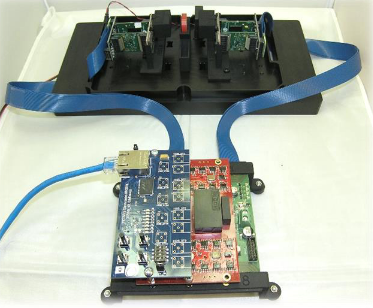
\includegraphics[scale=0.8]{3DesignPrinciples/32Tritium_detector/PETSYS_System.png}
\caption{Different parts of PETSYS system.\label{fig:PETSYS}~\cite{PETSYS}}
\end{figure}

Although the capacity provided by PETSYS should be enough for the requirements of the TRITIUM project, TRITIUM is a modular detector with scalable sensitivity. It means that, if an inprovement of its limits is needed to improve its sensitivity or to further reduce the background, more photosensors would be needed. Therefore, the electronic system should be able to increase its capacity in a scalable way. This requeriment is fulfilled by PETSYS since it has an additional module, called Clock and Trigger, to which up to sixteen different PETSYS basic boards can be connected. Theses sixteen PETsys basic boards are read in parallel, giving a total system capacity of reading 256 SiPM matrices (16384 SiPMs\footnote{$1024\cdot{}16 = 16384$}). 

PETSYS is based on C++ and Python scripts that are prepared for the main tasks required, such as time coincidence options between SiPM (or even SiPM matrices) or energy discrimination. It is open source, giving the possibility to modify the current scripts or develop others with additional functions. PETsys has a time resolution of $250~\pico\second$ which is one of the best time resolutions of commercial systems available and its price is around $10$\euro$/$ channel, which is cheaper compared to similar electronic systems.

As described in section \ref{sec:CharacterizationSiPM}, the SiPM matrix temperature is an important parameter. The PETsys system has the ability to monitor the temperature of the SiPM matrices and ASICS employed to control them. Temperature monitoring is important to ensure the correct functioning of both, photosensors and system. PETsys has the possibility of developing new scripts to implement the stability gain method reported in section \ref{sec:CharacterizationSiPM}.

Some characterization measurements was performed using the PETSYS system to ensure that the system works properly but most of the SiPM characterization work was carried out at the level of a single channel (individual SiPM).

It is important to start the characterizaton at the level of a single channel to reduce the uncertainties in the first results. In order to do so, an electronic system was designed, developed and built to read up to eight different SiPMs and to monitor their temperature.

This system consists of a PCB\footnote{PCB, Printed Circuit Board} which is used to provide the SiPM bias voltage and to read the SiPM output signal. An example of the electronic scheme (provided by Hamamatsu) in which this is based is shown in Figure \ref{fig:PCBSiPM}.

\begin{figure}
\centering
    \begin{subfigure}[b]{0.5\textwidth}
    \centering
    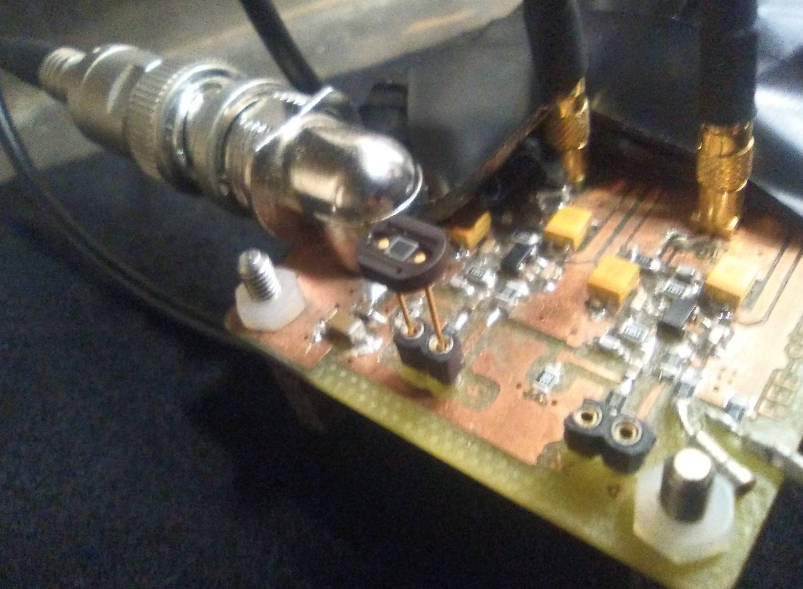
\includegraphics[width=\textwidth]{3DesignPrinciples/32Tritium_detector/SiPMPCB.png}  
    \caption{\label{subfig:ElectronicBoardSiPM}}
    \end{subfigure}
    \hfill
    \begin{subfigure}[b]{0.45\textwidth}
    \centering
    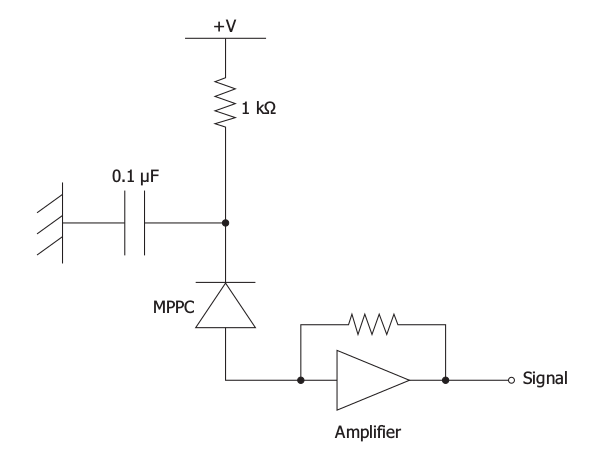
\includegraphics[width=\textwidth]{3DesignPrinciples/32Tritium_detector/ElectronicSchemePCBSiPM.png}  
    \caption{\label{subfig:ElectronicSchemePCBSiPM}}
    \end{subfigure}
    \hfill
 \caption{a) Electronic board used to provide the SiPM bias voltage and to read the SiPM output signal. b) Electronical scheme in which this PCB is based}
 \label{fig:PCBSiPM}
\end{figure}

The PCB was feed at $\pm6~\volt$ using the voltage source ISOTECH, model IPS-4303 \cite{VoltageSourceISOTECH} and the SiPM was feed using the electrometer KETHLEY, model 6517B \cite{VoltageSourceKethley}, with which a resolution of $1~\milli\volt$ is achieved, low enough to ensure that this does not affect to the SiPM gain.

The output signal of this PCB is connected to an oscilloscope, model WwaveRunner 625Zi from TELEDYNE LECROY \cite{OscilloscopeIFIMED} that records the data which are subsequently analized by ROOT\footnote{ROOT is a framework for data processing, based on C ++ and object-oriented technology, developed at CERN and widely used in nuclear and particle physics.}.